\documentclass[12pt,twocolumn ]{article}
\usepackage[utf8]{inputenc}
\usepackage{amsmath}
\usepackage{amssymb}
\usepackage{multirow}
\usepackage{fullpage}
\usepackage{graphicx}
\usepackage{amsthm}
\usepackage{makeidx}
\title{The God of Gentle-men's Game}
\author{Shubham Sharma}
\date{\today}
\makeindex
\begin{document}
\onecolumn
\maketitle
\tableofcontents
\listoffigures
\listoftables
\newpage
\twocolumn
\section{Introduction}
\par Sachin Tendulkar has been the most complete \index{batsman} of his time, the most \index{prolific} runmaker of all time, and \index{arguably} the biggest cricket icon the game has ever known. His \index{batting} was based on the purest \index{principles}: perfect balance, economy of movement, precision in \index{stroke-making}, and that \index{intangible} quality given only to \index{geniuses} - \index{anticipation}. If he didn't have a signature stroke - the upright, back-foot punch comes close - it's because he was equally proficient at each of the full range of orthodox shots (and plenty of improvised ones as well) and can pull them out at will.\par Blessed with the keenest of cricket minds, and armed with a loathing for losing, He set about doing what it took to become one of the best batsmen in the world. His greatness was established early: he was only 16 when he made his Test debut. He was hit on the mouth by Waqar Younis but continued to bat, in a blood-soaked shirt. His first Test hundred, a match-saving one at Old Trafford, came when he was 17, and he had 16 Test hundreds before he turned 25. In 2000 he became the first batsman to have scored 50 international hundreds, in 2008 he passed Brian Lara as the leading Test run-scorer, and in the years after, he went past 13,000 Test runs 30,000 international runs, and 50 Test hundreds.\par He currently holds the record for most hundreds in both Tests and ODIs - remarkable, considering he didn't score his first ODI hundred till his 79th match. Incredibly, he retained a divine enthusiasm for the game till his last match. At 36 years and 306 days he broke a 40-year-old barrier by scoring the first double-century in one-day cricket. In 2012, when just one month short of his 39th birthday, he became the first player to score 100 international centuries, which like Bradman's batting average, could be a mark that lasts for ever. Later that year, though, he announced his retirement from ODIs after a disappointing 18 months in international cricket. And on November 16, 2013, Tendulkar retired from Test cricket after a memorable 200th Test, on his home ground at the Wankhede Stadium against West Indies.His considerable achievements seem greater still when looked at in the light of the burden of expectations he had to bear from his adoring but somewhat unreasonable followers, who have been prone to regard anything less than a hundred in each innings as a failure. The aura may have dimmed, if only slightly, as the years on the international circuit took their toll on the body, but Tendulkar remains, by a distance, the most worshipped cricketer in the world\cite{sambit}.
\par Following are some true lines on Sachin
\par
\textit{Commit all your sins when Sachin is batting. They will go unnoticed because even the lord is watching!}
\par
Beneath the helmet, under that unruly curly hair, inside the cranium, there is something we don't know, something beyond scientific measure. Something that allows him to soar, to roam a territory of sport that, forget us, even those who are gifted enough to play alongside him cannot even fathom. When he goes out to bat, people switch on their TV sets and switch off their lives
\par
\textit{On a train from Shimla to Delhi, there was a halt in one of the stations. The train stopped by for few minutes as usual. Sachin was nearing century, batting on 98. The passengers, railway officials, everyone on the train waited for Sachin to complete the century. This Genius can stop time in India!}\cite{quora}
\par
\textit{I'll see god when I die but till then I'll see Sachin}
\onecolumn
\begin{figure*}[h]
        \begin{center}
                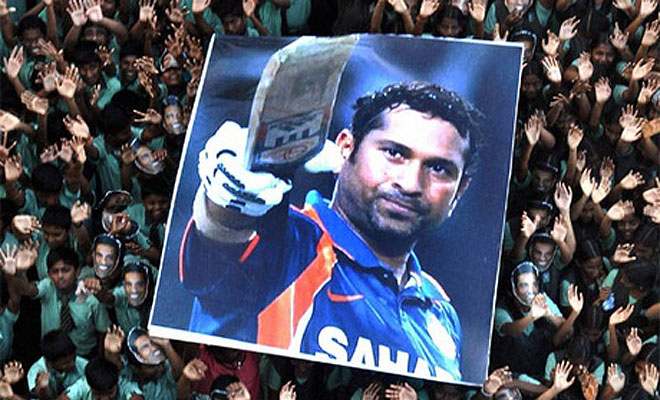
\includegraphics[scale=0.7]{index}
        \end{center}
        \caption{Fan Following}
        \label{fig:shapes}
\end{figure*}
\section{Carrier Statistics}
\par When your career spans several years, there is a lot to adapt to. Training, technology, techniques, styles - your own and your opponent's. It takes a special kind of person to conquer such dynamic challenges and continue performing at such a high level.\cite{quora}
\subsection{Batting and Fielding Averages}
\begin{table}[h]
    \centering
    \begin{tabular}{|c|c|c|c|c|c|c|c|c|c|c|}
     \hline
     Format & Mat & Inns & Runs & HS & Ave & SR & 100 & 50 & 4s & 6s  \\
     \hline
     Tests & 200 & 329 & 15921 & 248* & 53.78 & 87 & 51 & 68 & 1024 & 600 \\
     \hline
     ODIs & 463 & 452 & 18426 & 200* & 44.83 & 86.23 & 49 & 96 & 2016 & 195\\
     \hline
     First-class & 310 & 490 & 25396 & 248* & 57.84 & 89 & 81 & 116 & 1186 & 200\\
     \hline
     List A & 551 & 538 & 21999 & 200* & 45.54 &83& 60 & 114 & 1895 & 175\\
     \hline
     Twenty20 & 96  & 96 & 2797 & 100* & 32.90 & 121.08 & 1 & 16 & 359 & 38\\
     \hline
\end{tabular}
    \caption{Batting and Fielding Average}
    \label{tab:my_label}
\end{table}
\subsection{Bowling Averages}
\begin{table}[h]
    \centering
    \begin{tabular}{|c|c|c|c|c|c|c|c|c|c|c|c|}
    \hline
     Format & Mat &	Inns &	Balls &	Runs &	Wkts &	BBI &	BBM &	Ave &	Econ &	SR & 5w \\
     \hline
      Tests & 200 &	145 & 4240 & 2492 &	46 & 3/10 &	3/14 & 54.17 & 3.52 &	92.1 & 0 \\
      \hline
      ODIs & 463 & 270 & 8054 & 6850 & 154 & 5/32 & 5/32 & 44.48 & 5.10 & 52.2 & 4 \\
      \hline
      Twenty20 & 96 &	8 &	93 &	123 &	2 &	1/12 &	1/12 &	61.50 &	7.93 &	46.5 &	0 \\
      \hline
\end{tabular}
    \caption{Bowling Averages}
    \label{tab:my_label}
\end{table}
\subsection{Performance in big matches and chasing in ODI}
\begin{table}[h]
    \centering
    \begin{tabular}{|c|c|c|c|c|c|c|}
\hline
   
Batsman & ODI avg & ODI SR & Final avg & Final SR & Chase avg & Chase SR\\
\hline     
Sachin & 44.83 & 86.23 & 54.44 & 87.68 & 42.3 & 88.44\\
\hline
Dravid  & 39.16 & 71.24 & 34.71  & 68.13 & 35.2 & 68.78\\
\hline
Ponting & 42.03 &  80.39 & 38.42 & 82.21  & 41.93 &  76.34\\
\hline
Lara & 40.48 & 79.51 & 28.16 & 71.61 & 42.7 & 78.11\\
\hline
\end{tabular}
    \caption{Performance Comparison}
    \label{tab:my_label}
\end{table}
\subsection{Better away and fast bowling friendly wicket test record}
\begin{table}[h]
    \centering
    \begin{tabular}{|c|c|c|c|c|}
     \hline
     Batsman & In Australia & In England & In South Africa & In Away  \\
     \hline
     Sachin  & 53.20 & 54.31 & 46.44 & 54.74 \\
     \hline
     Ponting & 58.95 & 41.79 & 46.85 & 45.81\\
     \hline
     Dravid & 41.64 & 68.80 & 29.71 & 53.03\\
     \hline
     Lara & 41.97 & 48.76 & 46.72 & 47.80\\
     \hline
\end{tabular}
    \caption{Records}
    \label{tab:my_label}
\end{table}
\par  while overall average and strike rate of Sachin is higher than his peers, he still increases them in final matches. And except in Chase avg column he is at top in all others columns. Yes, he failed in two WC finals but he still has scored 31, 53 in 2 WC QFs and 65, 83, 85 in 3 WC SFs\cite{espn}.
\subsection{Better record against Australia(most dominating team during his time)}
\begin{table}[h]
    \centering
    \begin{tabular}{|c|c|c|}
    \hline
     Batsman & ODI avg & Test avg\\
    \hline
     Sachin  & 44.50 & 57.30\\
     \hline
     Dravid & 24.97 & 39.33\\
     \hline
     Lara & 39.50 & 51.00\\
     \hline
\end{tabular}
    \caption{Average Comparison}
    \label{tab:my_label}
\end{table}
\par Cricket has seen many greats come and go, but very few would argue that anyone came close to Sachin Tendulkar. The whole of India prayed for him every time he took his stance at the crease\cite{siddhartha}.
\par He is the most complete batsman ever. He played every stroke with equal perfection, he is equally good on both sides of the wicket ..you cannot just look at one stroke and say this is Sachin's best, his strokes are just memorable be it he pull against Caddick  or the straight drives  against \index{kasprowicz}, from the \index{orthodox} style of the 90's he has adapted his game to the modern style including the \index{paddle sweeps} and the \index{upper cuts}( he plays them better than anybody else), and above all what separates the great from the very best is the humility, no confrontations no flambuoyancy, he always let his bat do the talking\cite{harsha}.
\begin{figure*}[h]
        \begin{center}
                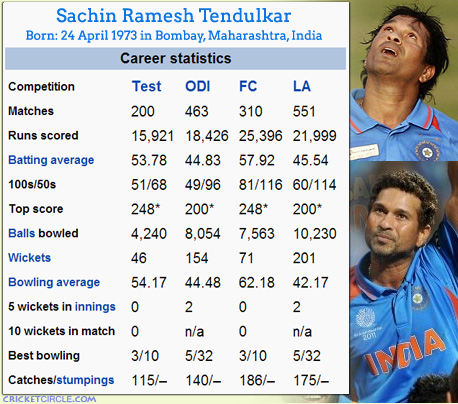
\includegraphics[scale=0.7]{sachin-career}
        \end{center}
        \caption{Records}
        \label{fig:shapes}
\end{figure*}
\newpage
\printindex
\medskip
\bibliographystyle{unsrt}
\bibliography{ex}





\end{document}
